\documentclass[10pt,a4paper]{report}
\usepackage[utf8]{inputenc}
\usepackage{amsmath}
\usepackage{amsfonts}
\usepackage{amssymb}
\usepackage{amsthm}
\usepackage{hyperref}
\usepackage{wasysym}

\usepackage{multicol}
\usepackage{fancyhdr}
\usepackage{enumitem}
\usepackage{tikz}
\usepackage{tikz-cd}
\usetikzlibrary{calc}
\usetikzlibrary{shapes.geometric}
\usepackage[margin=0.5in]{geometry}
\usepackage{xcolor}
\DeclareMathOperator{\RANGE}{range}
\DeclareMathOperator{\NULL}{null}

\hypersetup{
    colorlinks=true,
    linkcolor=blue,
    filecolor=magenta,      
    urlcolor=cyan,
    pdftitle={Tensors},
    pdfpagemode=FullScreen,
    }

%\urlstyle{same}

\newcommand{\CLASSNAME}{Functional Analysis}
\newcommand{\STUDENTNAME}{Paul Carmody}
\newcommand{\ASSIGNMENT}{Assignment \#1}
\newcommand{\DUEDATE}{February 15, 2024}
\newcommand{\SEMESTER}{Summer 2023}
\newcommand{\SCHEDULE}{T/Th 2:00 -- 3:20}
\newcommand{\ROOM}{Remote}

\pagestyle{fancy}
\fancyhf{}
\chead{ \fancyplain{}{\CLASSNAME} }
%\chead{ \fancyplain{}{\STUDENTNAME} }
\rhead{\thepage}
\newcommand{\LET}{\text{Let }}
%\newcommand{\IF}{\text{if }}
\newcommand{\AND}{\text{ and }}
\newcommand{\OR}{\text{ or }}
\newcommand{\FORSOME}{\text{ for some }}
\newcommand{\FORALL}{\text{ for all }}
\newcommand{\WHERE}{\text{ where }}
\newcommand{\WTS}{\text{ WTS }}
\newcommand{\WLOG}{\text{ WLOG }}
\newcommand{\BS}{\backslash}
\newcommand{\DEFINE}[1]{\textbf{\emph{#1}}}
\newcommand{\IF}{$(\Rightarrow)$}
\newcommand{\ONLYIF}{$(\Leftarrow)$}
\newcommand{\ITH}{\textsuperscript{th} }
\newcommand{\FST}{\textsuperscript{st} }
\newcommand{\SND}{\textsuperscript{nd} }
\newcommand{\TRD}{\textsuperscript{rd} }
\newcommand{\INV}{\textsuperscript{-1} }

\newcommand{\XXX}{\mathfrak{X}}
\newcommand{\MMM}{\mathfrak{M}}
%\newcommand{\????}{\textfrak{A}}
%\newcommand{\????}{\textgoth{A}}
%\newcommand{\????}{\textswab{A}}

\DeclareMathOperator{\DER}{Der}
\DeclareMathOperator{\SGN}{sgn}

%%%%%%%
% derivatives
%%%%%%%

\newcommand{\PART}[2]{\frac{\partial #1}{\partial #2}}
\newcommand{\SPART}[2]{\frac{\partial^2 #1}{\partial #2^2}}
\newcommand{\DERIV}[2]{\frac{d #1}{d #2}}
\newcommand{\LAPLACIAN}[1]{\frac{\partial^2 #1}{\partial x^2} + \frac{\partial^2 #1}{\partial y^2}}

%%%%%%%
% sum, product, union, intersections
%%%%%%%

\newcommand{\SUM}[2]{\underset{#1}{\overset{#2}{\sum}}}
\newcommand{\PROD}[2]{\underset{#1}{\overset{#2}{\prod}}}
\newcommand{\UNION}[2]{\underset{#1}{\overset{#2}{\bigcup}}}
\newcommand{\INTERSECT}[2]{\underset{#1}{\overset{#2}{\bigcap}}}
\newcommand{\FSUM}{\SUM{n=-\infty}{\infty}}
       

%%%%%%%
% supremum and infimum
%%%%%%%

\newcommand{\SUP}[1]{\underset{#1}\sup \,}
\newcommand{\INF}[1]{\underset{#1}\inf \,}
\newcommand{\MAX}[1]{\underset{#1}\max \,}
\newcommand{\MIN}[1]{\underset{#1}\min \,}

%%%%%%%
% infinite sums, limits
%%%%%%%

\newcommand{\SUMK}{\SUM{k=1}{\infty}}
\newcommand{\SUMN}{\SUM{n=1}{\infty}}
\newcommand{\SUMKZ}{\SUM{k=0}{\infty}}
\newcommand{\LIM}[1]{\underset{#1}\lim\,}
\newcommand{\IWOB}[1]{\LIM{#1 \to \infty}}
\newcommand{\LIMK}{\IWOB{k}}
\newcommand{\LIMN}{\IWOB{n}}
\newcommand{\LIMX}{\IWOB{x}}
\newcommand{\NIWOB}{\LIM{n \to \infty}}
\newcommand{\LIMSUPK}{\underset{k\to\infty}\limsup \,}
\newcommand{\LIMSUPN}{\underset{n\to\infty}\limsup \,}
\newcommand{\LIMINFK}{\underset{k\to\infty}\liminf \,}
\newcommand{\LIMINFN}{\underset{n\to\infty}\liminf \,}
\newcommand{\ROOTRULE}[1]{\LIMSUPK \BARS{#1}^{1/k}}

\newcommand{\CUPK}{\bigcup_{k=1}^{\infty}}
\newcommand{\CAPK}{\bigcap_{k=1}^{\infty}}
\newcommand{\CUPN}{\bigcup_{n=1}^{\infty}}
\newcommand{\CAPN}{\bigcap_{n=1}^{\infty}}

%%%%%%%
% number systems (real, rational, etc.)
%%%%%%%

\newcommand{\REALS}{\mathbb{R}}
\newcommand{\RATIONALS}{\mathbb{Q}}
\newcommand{\IRRATIONALS}{\REALS \backslash \RATIONALS}
\newcommand{\INTEGERS}{\mathbb{Z}}
\newcommand{\NUMBERS}{\mathbb{N}}
\newcommand{\COMPLEX}{\mathbb{C}}
\newcommand{\DISC}{\mathbb{D}}
\newcommand{\HPLANE}{\mathbb{H}}

\newcommand{\R}{\mathbb{R}}
\newcommand{\Q}{\mathbb{Q}}
\newcommand{\Z}{\mathbb{Z}}
\newcommand{\N}{\mathbb{N}}
\newcommand{\C}{\mathbb{C}}
\newcommand{\T}{\mathbb{T}}
\newcommand{\COUNTABLE}{\aleph_0}
\newcommand{\UNCOUNTABLE}{\aleph_1}


%%%%%%%
% Arithmetic/Algebraic operators
%%%%%%%


\DeclareMathOperator{\MOD}{mod}
%\newcommand{\MOD}[1]{\mod #1}
\newcommand{\BAR}[1]{\overline{#1}}
\newcommand{\LCM}{\text{ lcm}}
\newcommand{\ZMOD}[1]{\Z/#1\Z}
\DeclareMathOperator{\VAR}{Var}
%%%%%%%
% complex operators
%%%%%%%

\DeclareMathOperator{\RR}{Re}
%\newcommand{\RE}{\text{Re}}
\DeclareMathOperator{\IM}{Im}
%\newcommand{\IM}{\text{Im}}
\newcommand{\CONJ}[1]{\overline{#1}}
\DeclareMathOperator{\LOG}{Log}
%\newcommand{\LOG}{\text{ Log }}
\newcommand{\RES}[2]{\underset{#1}{\text{res}} #2}

%%%%%%%
% Group operators
%%%%%%%

\newcommand{\AUT}{\text{Aut}\,}
\newcommand{\KER}{\text{ker}\,}
\newcommand{\END}{\text{End}}
\newcommand{\HOM}{\text{Hom}}
\newcommand{\CYCLE}[1]{(\begin{array}{cccccccccc}
		#1
	\end{array})}
\newcommand{\SUBGROUP}{\underset{\text{group}}\subseteq}	
%\newcommand{\SUBGROUP}{\subseteq_g}
\newcommand{\SUBRING}{\underset{\text{ring}}\subseteq}
\newcommand{\SUBMOD}{\underset{\text{mod}}\subseteq}
\newcommand{\SUBFIELD}{\underset{\text{field}}\subseteq}
\newcommand{\ISO}{\underset{\text{iso}}\longrightarrow}
\newcommand{\HOMO}{\underset{\text{homo}}\longrightarrow}

%%%%%%%
% grouping (parenthesis, absolute value, square, multi-level brackets).
%%%%%%%

\newcommand{\PAREN}[1]{\left (\, #1 \,\right )}
\newcommand{\BRACKET}[1]{\left \{\, #1 \,\right \}}
\newcommand{\SQBRACKET}[1]{\left [\, #1 \,\right ]}
\newcommand{\ABRACKET}[1]{\left \langle\, #1 \,\right \rangle}
\newcommand{\BARS}[1]{\left |\, #1 \,\right |}
\newcommand{\DBARS}[1]{\left \| \, #1 \,\right \|}
\newcommand{\LBRACKET}[1]{\left \{ #1 \right .} 
\newcommand{\RBRACKET}[1]{\left . #1 \right \]}
\newcommand{\RBAR}[1]{\left . #1 \, \right |}
\newcommand{\LBAR}[1]{\left | \, #1 \right .}
\newcommand{\BLBRACKET}[2]{\BRACKET{\RBAR{#1}#2}}
\newcommand{\GEN}[1]{\ABRACKET{#1}}
\newcommand{\BINDEF}[2]{\LBRACKET{\begin{array}{ll}
     #1\\
     #2
\end{array}}}

%%%%%%%
% Fourier Analysis
%%%%%%%

\newcommand{\ONEOTWOPI}{\frac{1}{2\pi}}
\newcommand{\FHAT}{\hat{f}(n)}
\newcommand{\FINT}{\int_{-\pi}^\pi}
\newcommand{\FINTWO}{\int_{0}^{2\pi}}
\newcommand{\FSUMN}[1]{\SUM{n=-#1}{#1}}
%\newcommand{\FSUM}{\SUMN{\infty}}
\newcommand{\EIN}[1]{e^{in#1}}
\newcommand{\NEIN}[1]{e^{-in#1}}
\newcommand{\INTALL}{\int_{-\infty}^{\infty}}
\newcommand{\FTINT}[1]{\INTALL #1 e^{2\pi inx\xi} dx}
\newcommand{\GAUSS}{e^{-\pi x^2}}

%%%%%%%
% formatting 
%%%%%%%

\newcommand{\LEFTBOLD}[1]{\noindent\textbf{#1}}
\newcommand{\SEQ}[1]{\{#1\,\}}
\newcommand{\WIP}{\footnote{work in progress}}
\newcommand{\QED}{\hfill\square}
\newcommand{\ts}{\textsuperscript}
\newcommand{\HLINE}{\noindent\rule{7in}{1pt}\\}

%%%%%%%
% Mathematical note taking (definitions, theorems, etc.)
%%%%%%%

\newcommand{\REM}{\noindent\textbf{\\Remark: }}
\newcommand{\DEF}{\noindent\textbf{\\Definition: }}
\newcommand{\THE}{\noindent\textbf{\\Theorem: }}
\newcommand{\COR}{\noindent\textbf{\\Corollary: }}
\newcommand{\LEM}{\noindent\textbf{\\Lemma: }}
\newcommand{\PROP}{\noindent\textbf{\\Proposition: }}
\newcommand{\PROOF}{\noindent\textbf{\\Proof: }}
\newcommand{\EXP}{\noindent\textbf{\\Example: }}
\newcommand{\TRICKS}{\noindent\textbf{\\Tricks: }}


%%%%%%%
% text highlighting
%%%%%%%

\newcommand{\B}[1]{\textbf{#1}}
\newcommand{\CAL}[1]{\mathcal{#1}}
\newcommand{\UL}[1]{\underline{#1}}

%%%%%%
% Linear Algebra
%%%%%%

\newcommand{\COLVECTOR}[1]{\PAREN{\begin{array}{c}
#1
\end{array} }}
\newcommand{\TWOXTWO}[4]{\PAREN{ \begin{array}{c c} #1&#2 \\ #3 & #4 \end{array} }}
\newcommand{\DTWOXTWO}[4]{\BARS{ \begin{array}{c c} #1&#2 \\ #3 & #4 \end{array} }}
\newcommand{\THREEXTHREE}[9]{\PAREN{ \begin{array}{c c c} #1&#2&#3 \\ #4 & #5 & #6 \\ #7 & #8 & #9 \end{array} }}
\newcommand{\DTHREEXTHREE}[9]{\BARS{ \begin{array}{c c c} #1&#2&#3 \\ #4 & #5 & #6 \\ #7 & #8 & #9 \end{array} }}
\newcommand{\NXN}{\PAREN{ \begin{array}{c c c c} 
			a_{11} & a_{12} & \cdots & a_{1n} \\
			a_{21} & a_{22} & \cdots & a_{2n} \\
			\vdots & \vdots & \ddots & a_{1n} \\
			a_{n1} & a_{n2} & \cdots & a_{nn} \\
		\end{array} }}
\newcommand{\SLR}{SL_2(\R)}
\newcommand{\GLR}{GL_2(\R)}
\DeclareMathOperator{\TR}{tr}
\DeclareMathOperator{\BIL}{Bil}
\DeclareMathOperator{\SPAN}{span}

%%%%%%%
%  White space
%%%%%%%

\newcommand{\BOXIT}[1]{\noindent\fbox{\parbox{\textwidth}{#1}}}


\newtheorem{theorem}{Theorem}[section]
\newtheorem{corollary}{Corollary}[theorem]
\newtheorem{lemma}[theorem]{Lemma}

\theoremstyle{definition}
\newtheorem{definition}[theorem]{Definition}
\newtheorem{prop}[theorem]{Proposition}

\theoremstyle{remark}
\newtheorem{remark}[theorem]{Remark}
\newtheorem{example}[theorem]{Example}
%\newtheorem*{proof}[theorem]{Proof}



\newcommand{\RED}[1]{\textcolor{red}{#1}}
\newcommand{\BLUE}[1]{\textcolor{blue}{#1}}
\newcommand{\GREEN}[1]{\textcolor{black!30!green}{#1}}
\newcommand{\ORANGE}[1]{\textcolor{orange}{#1}}
\newcommand{\F}{\textbf{F}}

\title{Advanced Linear Algebra}
\author{The Unforgetable Someone}
\date{Summer 2023}

\newcommand{\NORM}[1]{\,\left \Vert #1 \right \Vert\,}
\begin{document}

\begin{center}
	\Large{\CLASSNAME -- \SEMESTER} \\
\end{center}
\begin{center}
	\STUDENTNAME \\
	\ASSIGNMENT -- \DUEDATE\\
\end{center} 
\vskip 0.5cm

Page. 65 \#11, \textbf{(Convex set, segment)}  A subset $A$ of a vector space $X$ is said to be \textit{convex} if $x,y \in A$ implies $$ M= \{z\in Z \,|\, z=\alpha x+(1-\alpha)y, \, 0\le \alpha\le 1\} \subset A $$ $M$ is called \textit{a closed segment} with \textit{boundary points} $x$ and $y$; any other $z \in M$ is called an \textit{interior point} of $M$.  Show that the \textit{closed unit ball}  $$ \tilde{B}(0;1)=\{x\in X\,|\,||x||\le 1\} $$ in a normed space $X$ is convex.\\
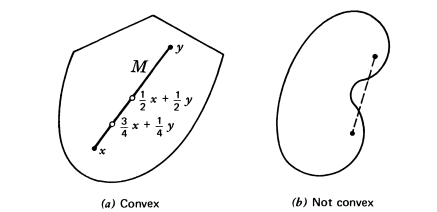
\includegraphics[scale=.7]{p65ex11.png} 
\\ \\
Let, $x,y \in \tilde{B}(0;1)$ which implies that $||x|| \le 1$ and $||y|| \le 1$.  Given any point $m \in M$ there exists $\alpha$ where $0\le \alpha \le 1$, such that $m=\alpha x + (1-\alpha)y$.  Thus, $||m|| = ||\alpha x + (1-\alpha)y||$
\begin{align*}
	\NORM{m} &= \NORM{\alpha x + (1-\alpha)y} \\
		&\le ||\alpha x|| + ||(1-\alpha)y||\\
		&\le |\alpha| \, ||x|| + |1-\alpha| \, ||y|| \\
	\text{Let } p &= \max(||x||,||y||) \\
	||m|| &\le |\alpha| \, p + |1-\alpha| \, p \\
		&\le (|\alpha| + |(1-\alpha)|)p \\
		&\le p \\
	\therefore m &\in \tilde{B}(0;1)
\end{align*}$x,y$ are arbitrary points and $m$ is an arbitrary point between them.  Hence, $\tilde{B}(0;1)$ must be convex.

\newpage
Page. 70 
\begin{enumerate}
	\item Show that $c \subset \ell^\infty$ is a vector space of $\ell^\infty$ (cf. 1.5-3) and so is $c_0$, the space of all sequences of scalars converging to zero.\\
	\\
	Given any $x,y \in \ell^\infty$ and $c_x, c_y$ are bounds for these sequences with $x = (\eta_j) \le c_x$ and $y=(\xi_j) \le c_y$.  Then given any $\alpha \in \C$ we have
	\begin{align*}
		\alpha(x + y) &= \alpha(\eta_j + \xi_j)_{j=1}^\infty & \text{component-wise addition} \\
		&= (\alpha\eta_j + \alpha\xi_j)_{j=1}^\infty \\
		|\alpha\eta_j + \alpha\xi_j|_{j=1}^\infty &\le |\alpha|(c_x + c_y)
	\end{align*}thus we have a new bounded sequence, that is $\alpha(x+y) \in \ell^\infty$.  Thus, $\ell^\infty$ is a vector space.\\ \\
	Notice that if $c_x = c_y = 0$ that $|\eta_j + \xi_j| \le c_x+c_y = 0$ for all $1 \le j < \infty$, thus $x+y \in c_0$.\\
	
	\item Show that $c_0$ in Prob 1 is a \textit{closed} subspace of $\ell^\infty$, so that $c_0$ is complete by 1.5-2 and 1.4-7. \\
	\\
	Let $x,y \in \ell^\infty \backslash c_0$ each converges to real numbers $c_x, c_y$, respectively.  Note that $c_x,c_y$ are strictly greater than zero.  Thus, $d(x,y) \le \max(c_x, c_y)$ and is distinctly not zero.  Hence, given any $\epsilon> 0$ there exists $B(x;\epsilon) \subset \ell^\infty\backslash c_0$.  Thus  $\ell^\infty\backslash c_0$ must be open which indicates that $c_0$ must be closed.\\
	
	\item In $\ell^\infty$, let $Y$ be the subset of all sequences with only finitely many nonzero terms.  Show that $Y$ is a subspace of $\ell^\infty$ but not a closed subspace. 
	
	\setcounter{enumi}{7}
	\item If in a normed space $X$, absolute convergence of any series always implies convergence of that series, show that $X$ is complete.
	
	\item Show that in a Banach space, an absolutely convergent series is convergent.
	
	\item \textbf{(Schauder basis)} Show that if a normed space has a Shauder basis, it is separable.
	
	\item Show that $(e_n)$, where $e_n=(\delta_{nj})$, is a Schauder basis for $\ell^p$, where $1 \le p < +\infty$.
	
	\setcounter{enumi}{14}
	\item \textbf{(Product of normed spaces)}  If $(X_1,||\cdot||_1)$ and $(X_2, ||\cdot||_2)$ are normed spaces, show that the product vector space $X=X_1\times X_2$ (cf. prob 13, Sec 2.1) becomes a normed space if we define
	\begin{align*}
		 ||x||=\max\PAREN{||x_1||_1, ||x_2||_2} \text{ where } x=(x_1, x_2).
	\end{align*}
\end{enumerate}

\newpage

Page. 76 \#1.  Give examples of subspaces of $\ell^\infty$ and $\ell^2$ which are not closed.

\LARGE{\textbf{$$ \BLUE{\boldsymbol{>}} \, \RED{\boldsymbol{\Sigma}^\Psi_{\male}}  \boldsymbol{\cdot} \GREEN{\text{C}^8_5} \, \BLUE{\boldsymbol{<}} $$}}\\
%\Large{$$ \left\rangle \, \Sigma^\Psi_{\male}  \boldsymbol{\cdot} \textlarge dot{C}^8_5 \, \right\langle $$}\\

\end{document}